\documentclass[letterpaper]{article} % DO NOT CHANGE THIS
\usepackage{aaai2027}  % DO NOT CHANGE THIS
\usepackage[hyphens]{url}  % DO NOT CHANGE THIS
\usepackage{graphicx} % DO NOT CHANGE THIS
\urlstyle{rm} % DO NOT CHANGE THIS
\def\UrlFont{\rm}  % DO NOT CHANGE THIS
\usepackage{natbib}  % DO NOT CHANGE THIS AND DO NOT ADD ANY OPTIONS TO IT
\usepackage{caption} % DO NOT CHANGE THIS AND DO NOT ADD ANY OPTIONS TO IT
\frenchspacing  % DO NOT CHANGE THIS
\usepackage{booktabs}
\usepackage{tikz}
\usetikzlibrary{positioning,arrows.meta}
\pdfinfo{
/TemplateVersion (2027.1)
}
\setcounter{secnumdepth}{0}

\title{ForeSight: Small Calibrated Decision Models as Opponent Forecasters\\for Lookahead Game Play}
\author{
    Saiakhil Chilaka
}
\affiliations{
    Cornell University\\
    314 West Ave, Ithaca, NY 14853\\
    (984) 260-2526\\
    sc3484@cornell.edu
}

\begin{document}

\maketitle

\begin{abstract}
To choose a good move, an agent has to guess how its opponent will respond. Game engines make that guess with hand-written rules and an exact simulator, which settings like negotiations do not have. LLM agents make it with large generative models, which are slow, poorly calibrated, and have little to no future sight. We propose ForeSight, which fine-tunes a small, non-generative ``System One'' decision model to give a calibrated probability for each opponent action, then uses those probabilities to weight every branch of a lookahead search. In Pok\'emon Showdown, a 421M-parameter forecaster trained for 35 minutes on a laptop, using only games between weak bots and at a much lower depth than its maximum potential, predicts the opponent's next action 72--80\% of the time (43\% zero-shot, 49\% for a damage-based rule). It reaches 75\% on an opponent it never saw in training, at 36--84\,ms per forecast. With no LLM, ForeSight wins 56.5\% of 200 games against the Abyssal benchmark bot. That matches the LLM agent PokéLLMon (56\%) but trails PokéChamp (64--70\%), and searching one extra turn ahead adds 13--20 points over one-step play. Every part is still minimal, so small calibrated forecasters could bring engine-style lookahead to settings with no engine.
\end{abstract}

\begin{links}
    \link{Code}{https://github.com/akhilc08/aaai-27}
\end{links}

\section{Introduction}
Good decisions, whether a move in a game or a step in negotiations, depend on predicting how the other side will react. Classical game engines do this with search over an exact simulator and a hand-written evaluator built for the engine. The Pok\'emon engine Foul Play, for example, pairs tree search with a hand-tuned position score \citep{foulplay}. That works when the rules are fully known, but it breaks down in negotiation and less deterministic settings, which have no simulator and no obvious hand-written opponent model.

LLM agents have different problems. In Pok\'emon Showdown, PokéLLMon asks an LLM to pick each move \citep{pokellmon}, and PokéChamp uses one to propose actions, model the opponent and score positions inside a minimax search \citep{pokechamp}. LLMs know a lot about the game, but their stated probabilities are poorly calibrated and each call takes seconds, an issue that hurts PokéChamp since it traces about a third of its losses to running out of turn time.

ForeSight splits the problem into two parts: a model that forecasts and a search that decides. The forecaster is a System One decision model \citep{jev,laya}. It reads a state and a list of typed options and returns a calibrated probability for each. A probability-weighted search then turns those forecasts into a move (Figure~\ref{fig:overview}). We test ForeSight in Pok\'emon Showdown since it combines hidden information, chance and a large action space, and has published LLM baselines.

\section{ForeSight}
\begin{figure}[t]
\centering
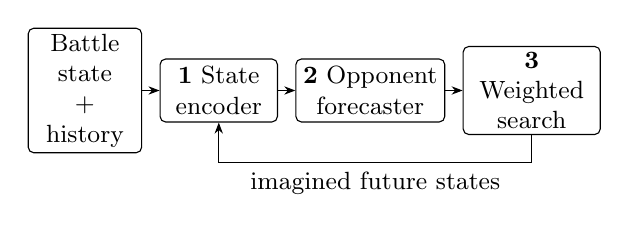
\begin{tikzpicture}[font=\small, node distance=2.2mm,
  box/.style={draw, rounded corners=2pt, align=center, inner sep=2pt, minimum height=8mm},
  arr/.style={-{Stealth[length=4pt]}}]
\node[box, text width=1.3cm] (s) {Battle state\\+ history};
\node[box, text width=1.35cm, right=of s] (e) {\textbf{1} State\\encoder};
\node[box, text width=1.75cm, right=of e] (f) {\textbf{2} Opponent\\forecaster};
\node[box, text width=1.6cm, right=of f] (x) {\textbf{3} Weighted\\search};
\draw[arr] (s) -- (e);
\draw[arr] (e) -- (f);
\draw[arr] (f) -- (x);
\draw[arr] (x.south) -- ++(0,-3.5mm) -| node[pos=0.25, below]{imagined future states} (e.south);
\end{tikzpicture}
\caption{ForeSight. The search weights every imagined future by the forecaster's opponent probabilities and by chance, then plays the best expected move.}
\label{fig:overview}
\end{figure}

\textbf{1. State encoder.} Each position is written out as short precomputed facts: units left, HP, who moves first, estimated damage, knock-out chances for each attack, type matchups, and both sides' last few actions. The opponent's candidate actions are its revealed moves, placeholders for unrevealed moves, and switches to Pok\'emon we have seen.

\textbf{2. Opponent forecaster.} We fine-tune Laya \citep{laya}, an open 421M-parameter System One model, on 10k opponent decisions sampled from 142k local games between simple rule-based and random bots (the data is weak since it comes from bots, not real players or better engines). We train the top four encoder layers and the decision head with Laya's proper-scoring-rule loss, then fit a temperature on validation data. Fine-tuning currently takes 35 minutes on an Apple M5 Pro MacBook.

\textbf{3. Probability-weighted search.} ForeSight runs a depth-2 expectimax. For each of our actions, it branches over the forecaster's distribution of opponent replies and over chance events (accuracy, damage rolls near a knock-out, secondary effects, speed ties), keeping 90\% of the probability mass at each node. Leaves are scored by the HP difference between the two sides (another deliberately weak design) and we play the action with the highest expected value.

\section{Evaluation}
\textbf{Experimental Setup.} We test forecasters trained on Gen 9 and Gen 8 games on held-out battles, and compare them with a rule that always predicts the opponent's strongest attack. For play, we follow PokéChamp's protocol: Gen 8 random battles without Dynamax against Abyssal, a rule-based bot that never appears in our training data, on a local Showdown server with a 15\,s turn limit.

\begin{table}[t]
\centering
\small
\begin{tabular}{llcc}
\toprule
Forecaster & Evaluated on & Acc. & Log-loss \\
\midrule
Damage-based rule & Gen 9 bots & 48.5\% & 1.24 \\
Laya, zero-shot & Gen 9 bots & 43.4\% & 1.15 \\
ForeSight (Gen 9) & Gen 9 bots & 71.8\% & 0.70 \\
ForeSight (Gen 8) & Gen 8 bots & \textbf{79.6\%} & \textbf{0.54} \\
\midrule
ForeSight (Gen 9) & Abyssal, unseen & 73.0\% & 0.62 \\
ForeSight (Gen 8) & Abyssal, unseen & 75.4\% & 0.58 \\
\bottomrule
\end{tabular}
\caption{Next-action forecasting on held-out turns ($n{=}$3,754--4,000 bot turns; 1,963 Abyssal turns).}
\label{tab:forecast}
\end{table}

\begin{table}[t]
\centering
\small
\begin{tabular}{llc}
\toprule
Agent & Decision model & Win rate \\
\midrule
PokéLLMon$^\dagger$ & GPT-4o & 56\% \\
PokéChamp$^\dagger$ & Llama-3.1-8B & 64\% \\
PokéChamp$^\dagger$ & GPT-4o & 70\% \\
\midrule
ForeSight (Gen 9) & Laya 421M & 56.5\% \\
ForeSight (Gen 8) & Laya 421M & 56.5\% \\
\bottomrule
\end{tabular}
\caption{Win rate against Abyssal. $^\dagger$Published by \citet{pokechamp}. ForeSight: $n{=}200$ games each, 95\% CI 50--63\%.}
\label{tab:play}
\end{table}

\textbf{Forecasting.} Fine-tuning turns a weak zero-shot model into an accurate, well-calibrated forecaster (calibration error 0.02; Table~\ref{tab:forecast}). It also transfers: on Abyssal, which it never saw in training, it predicts 73--75\% of actions.

\textbf{Play.} Without an LLM, ForeSight plays about as well as PokéLLMon with a far smaller model, though it trails PokéChamp (Table~\ref{tab:play}). The Gen 8 forecaster predicts better but wins no more often. Since the forecasts on Abyssal are already accurate, we think the gap to PokéChamp comes mostly from our shallow search and simple leaf.

\textbf{Speed and depth.} One forecast takes 36--84\,ms depending on batch size, and a turn takes 2.7--4.1\,s on average, so the 15\,s limit leaves room for 10--25$\times$ more search than we use. Lookahead clearly matters. Against Abyssal, searching a second turn ahead adds 13--20 points for every opponent model we tried (42\% to 58\%, $n{=}1000$ each), and our depth-1 result is in line with PokéChamp's one-step baseline (44\%). Outside games, in the text household benchmark ALFWorld \citep{alfworld}, letting a System One model pick among an LLM's top three actions by predicted outcome raised success from 34.6\% to 48.4\% ($p{<}0.001$).

\section{Conclusion and Future Work}
ForeSight uses a small, fine-tuned, calibrated decision model as the opponent forecaster inside a lookahead search. Even this bare-bones version matches an LLM agent built on a much larger model. Zero-shot System One models (Laya, and Jev in our pilots) forecast poorly, so fine-tuning is essential.

\textbf{Headroom.} Every component is simple and can improve.
(1)~\emph{Deeper search}: we use less than a tenth of the turn budget.
(2)~\emph{Better data}: trained only on weak bot games, the forecaster already predicts an unseen opponent 75\% of the time. Training on better data such as replays of high-rated human games \citep{metamon} should push that higher.
(3)~\emph{A learned leaf}: scoring by HP alone means setup moves, like Swords Dance, that benefit far into the future only count if their benefits land within two turns. A learned win-probability leaf could value essential parts of the game that are currently ignored.
(4)~\emph{Full fine-tuning and exact rules}: we train only 18\% of the parameters. A full fine-tune with sampled hidden teams would remove known simulator errors in the model.
Finally, since ForeSight needs no hand-written opponent model, we plan to apply it to negotiation \citep{dealornodeal} and other less deterministic environments, with an LLM proposing the candidate next states.

\section*{Acknowledgments}
Claude Code (Anthropic) assisted with experiment code, evaluation runs and editing; the author directed the work and is responsible for all content.

\bibliography{refs}

\end{document}
